Über die Navigationsleiste im oberen Bereich der Anwendung kann der/die Nutzer:in durch einen Klick auf "Fragenkonfigurator" direkt zum Fragenkonfigurator wechseln. Dort besteht die Möglichkeit, Fragen zu erstellen, zu bearbeiten und zu lernen.
\setauthor{\firstauthor}
\subsection{Übersicht}
\begin{figure}[h t]
    \centering
    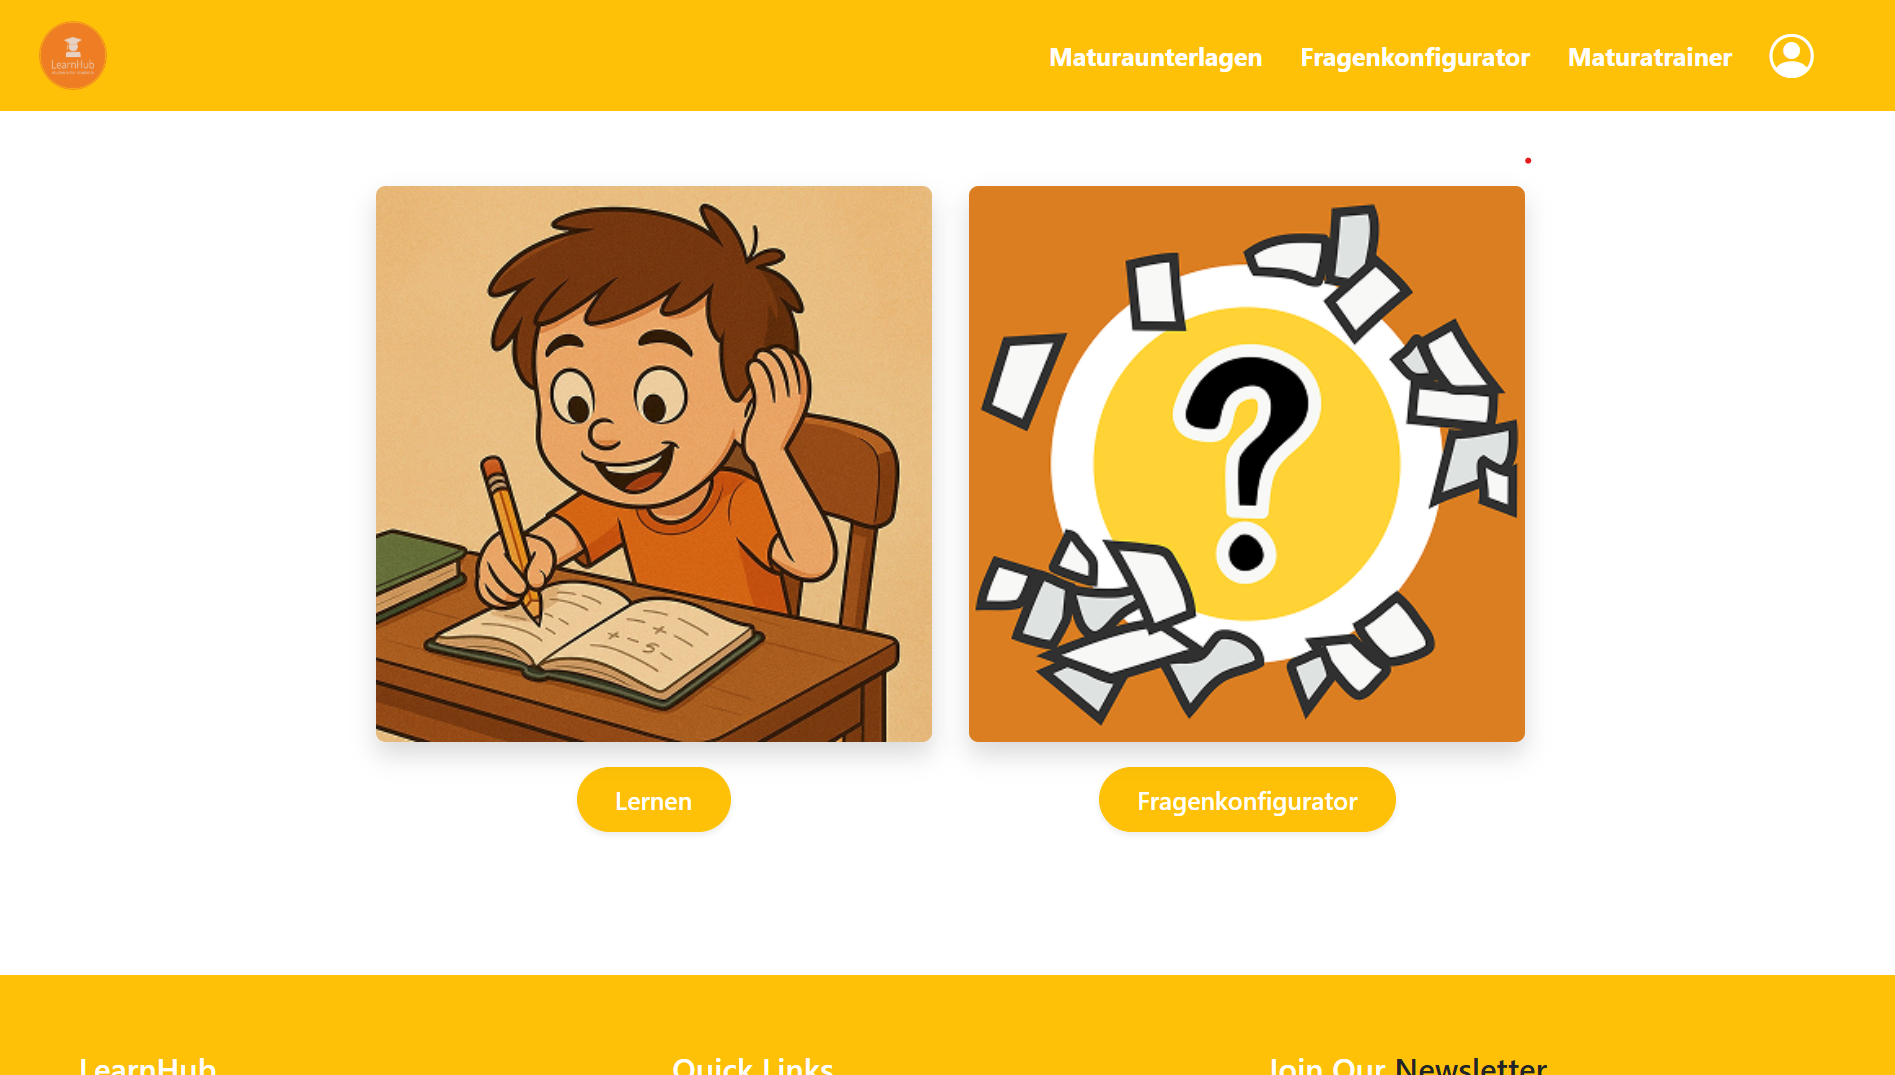
\includegraphics[width=0.6\textwidth]{pics/fragenkonf_auswahl.png}
    \caption{Auswahl: Lernen, Fragenkonfigurator}
\end{figure}
\subsubsection{Auswahl zwischen Lernmodus und Fragenkonfigurator}
Die Auswahl ermöglicht dem/der Nutzer:in, entweder in den Lernmodus zu wechseln oder den Fragenkonfigurator zur Erstellung und Verwaltung von Fragen zu nutzen. \par
Ein Klick auf "Lernen" führt zur Fachauswahl, in der alle verfügbaren Fächer angezeigt werden \ref{chapter:lernbereich}. \par
Ein Klick auf "Fragenkonfigurator" öffnet die Option Fragen zu Bearbeiten ("Erstellen" oder "Bearbeiten") \ref{chapter:fragen_verwalten}.

\subsection{Lernbereich} \label{chapter:lernbereich}
\begin{figure}[h t]
    \centering
    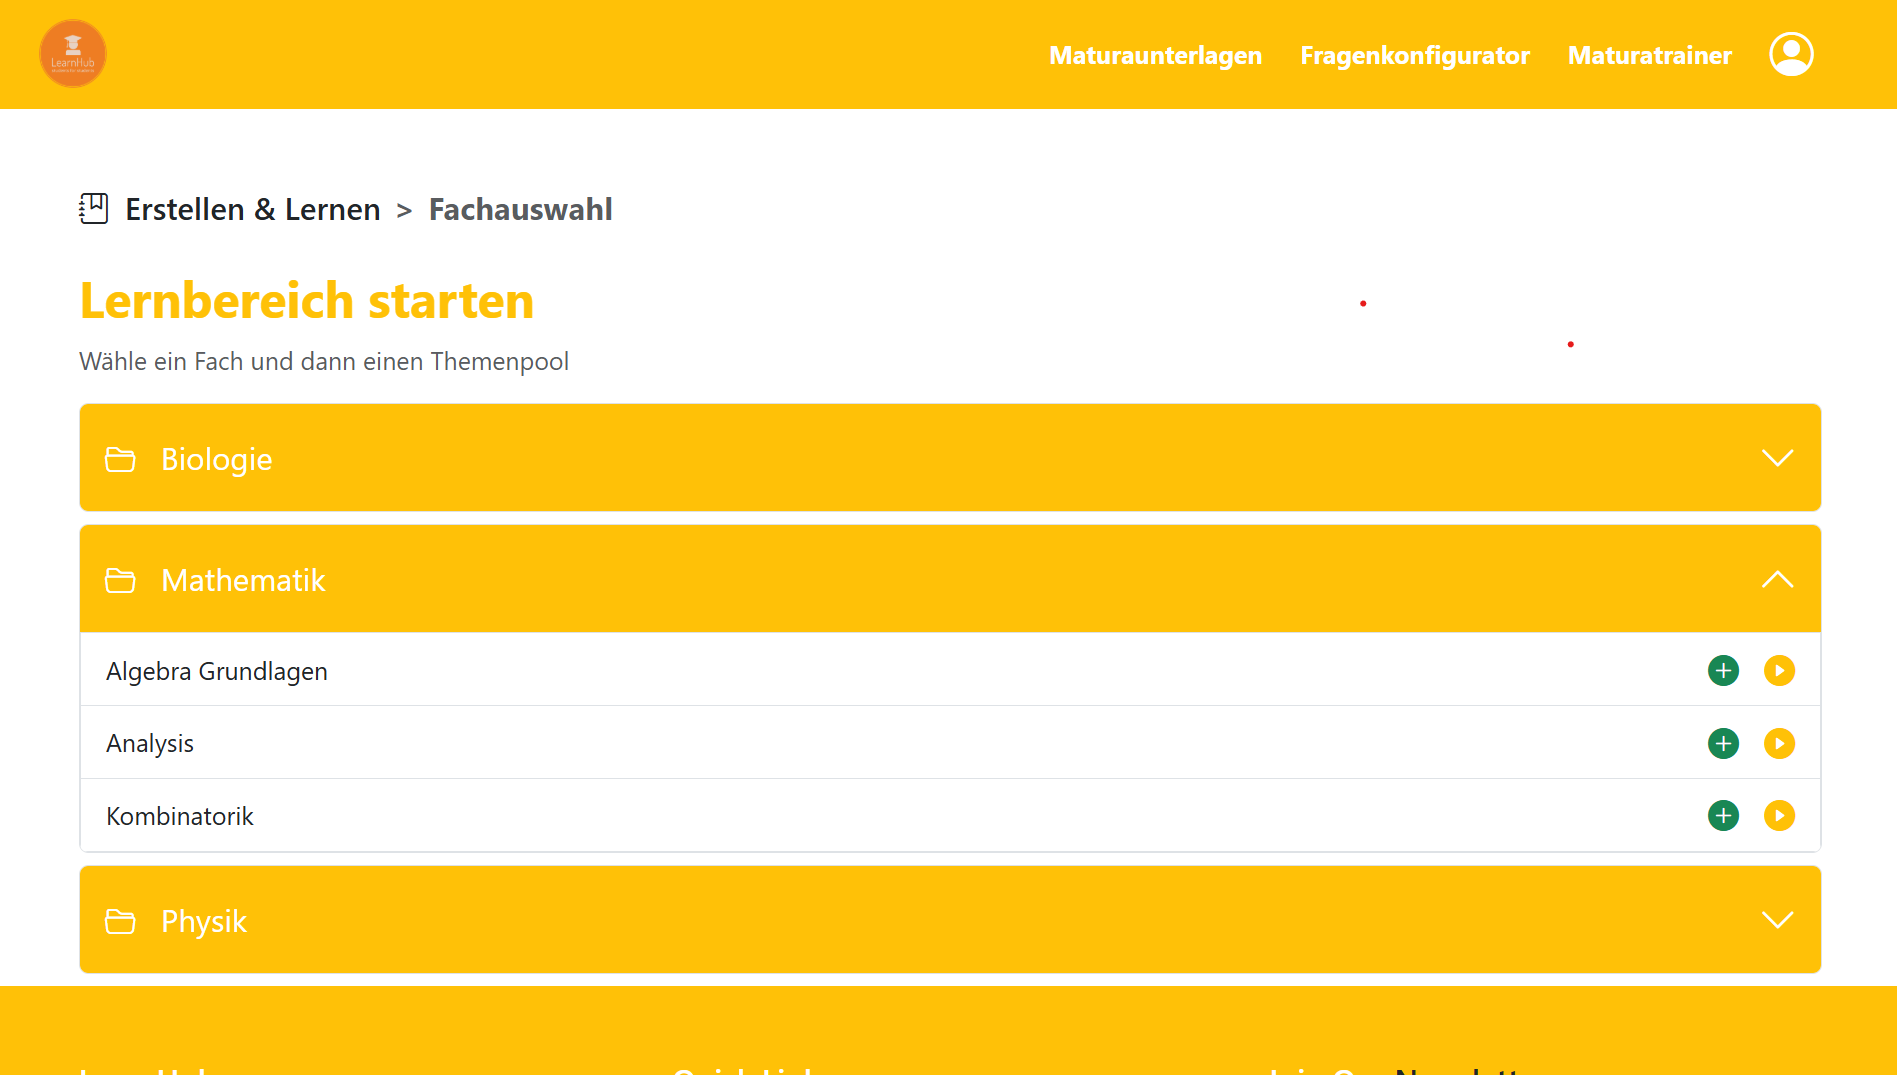
\includegraphics[width=0.6\textwidth]{pics/fragenkonf_lernen_fachauswahl.png}
    \caption{Lernbereich auswählen/Fachauswahl}
    \label{fig:lernbereich-auswahl}
\end{figure}

\subsubsection{Fachauswahl} \label{sec:fachauswahl}
In der Fachauswahl werden per Drop-Down-Menü die zugehörigen Themenpools angezeigt. Wechselt der/die Nutzer:in das Fach, wird der zuvor geöffnete Themenpool geschlossen.\par
Innerhalb eines geöffneten Themenpools stehen zwei Buttons zur Verfügung: ein grüner Kreis mit einem Plus (+) und ein orangener Kreis mit einem "Play"-Symbol.\par
Durch einen Klick auf den grünen Button gelangt der/die Nutzer:in zum Fragenkonfigurator, wobei Fach und Themenpool bereits vorausgewählt sind \ref{sec:frage-erstellen-vorausgewählt}. Der orangene Button führt zum Lernmodus \ref{sec:lernmodus}.\par

\begin{figure}[h t]
    \centering
    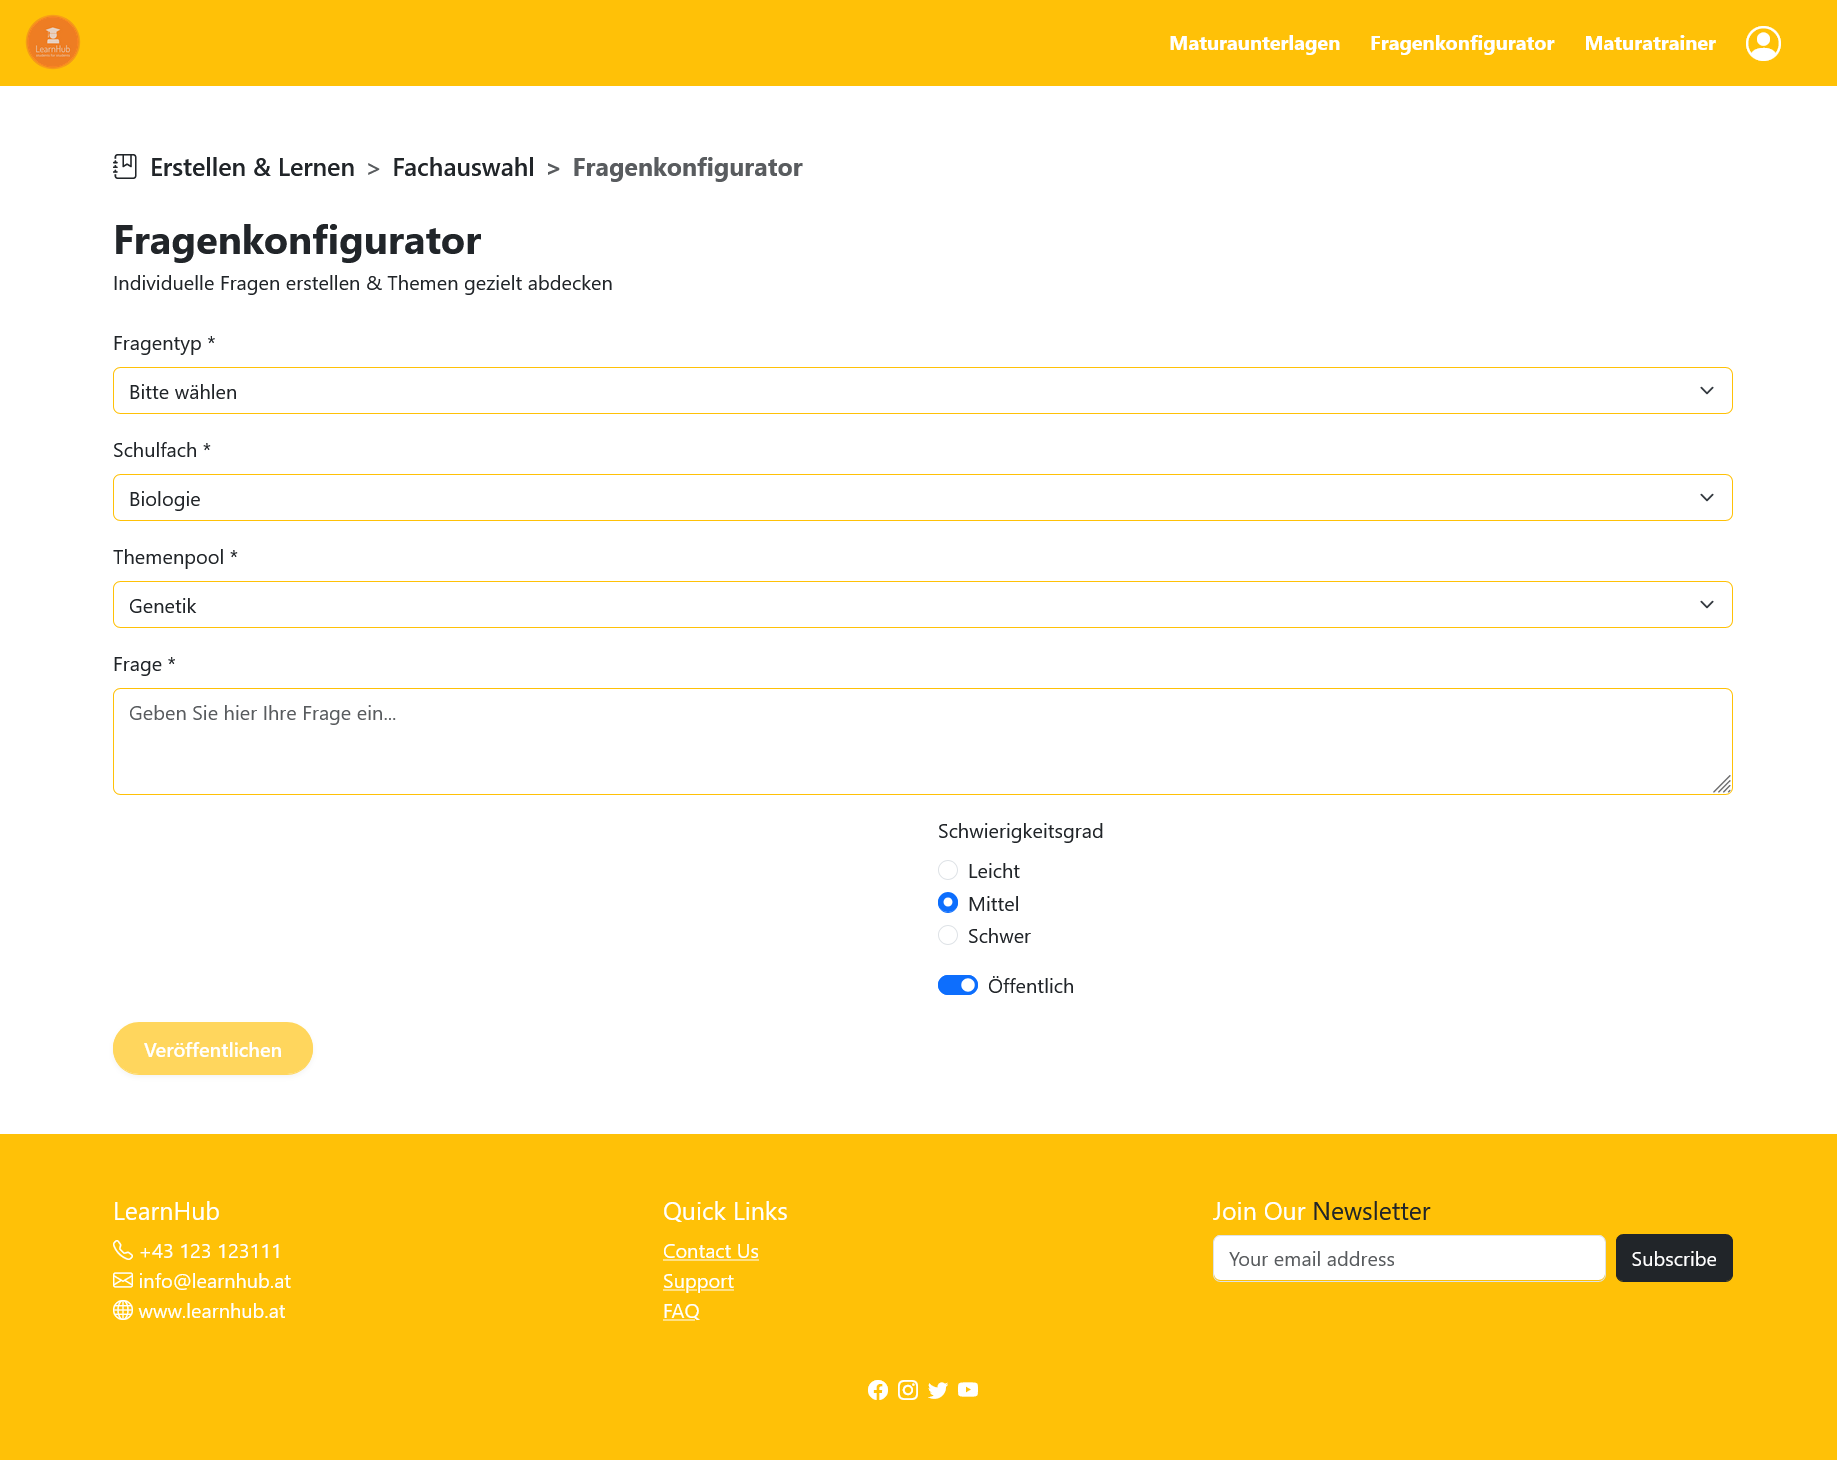
\includegraphics[width=0.6\textwidth]{pics/fragenkonf_erstellen_mit_fachauswahl.png}
    \caption{Fragenkonfigurator mit vorausgewähltem Fach und Themenpool}
    \label{fig:fragenkonfigurator-vorausgewählt}
\end{figure}
\subsubsection{Frage erstellen mit vorausgewähltem Fach und Themenpool} \label{sec:frage-erstellen-vorausgewählt}
Der/die Nutzer:in wählt den Fragetyp aus, formuliert die Frage, gibt die Antwortmöglichkeiten ein und markiert die korrekte Antwort. Nach Ausfüllen aller erforderlichen Felder kann die Frage durch einen Klick auf den "Veröffentlichen"-Button gespeichert werden. \par
Der Fragenkonfigurator wird im Kapitel xyz \ref{chapter:implementation} detalliert erläutert. % TODO: Kapitelnummer anpassen

\begin{figure}[H]
    \centering
    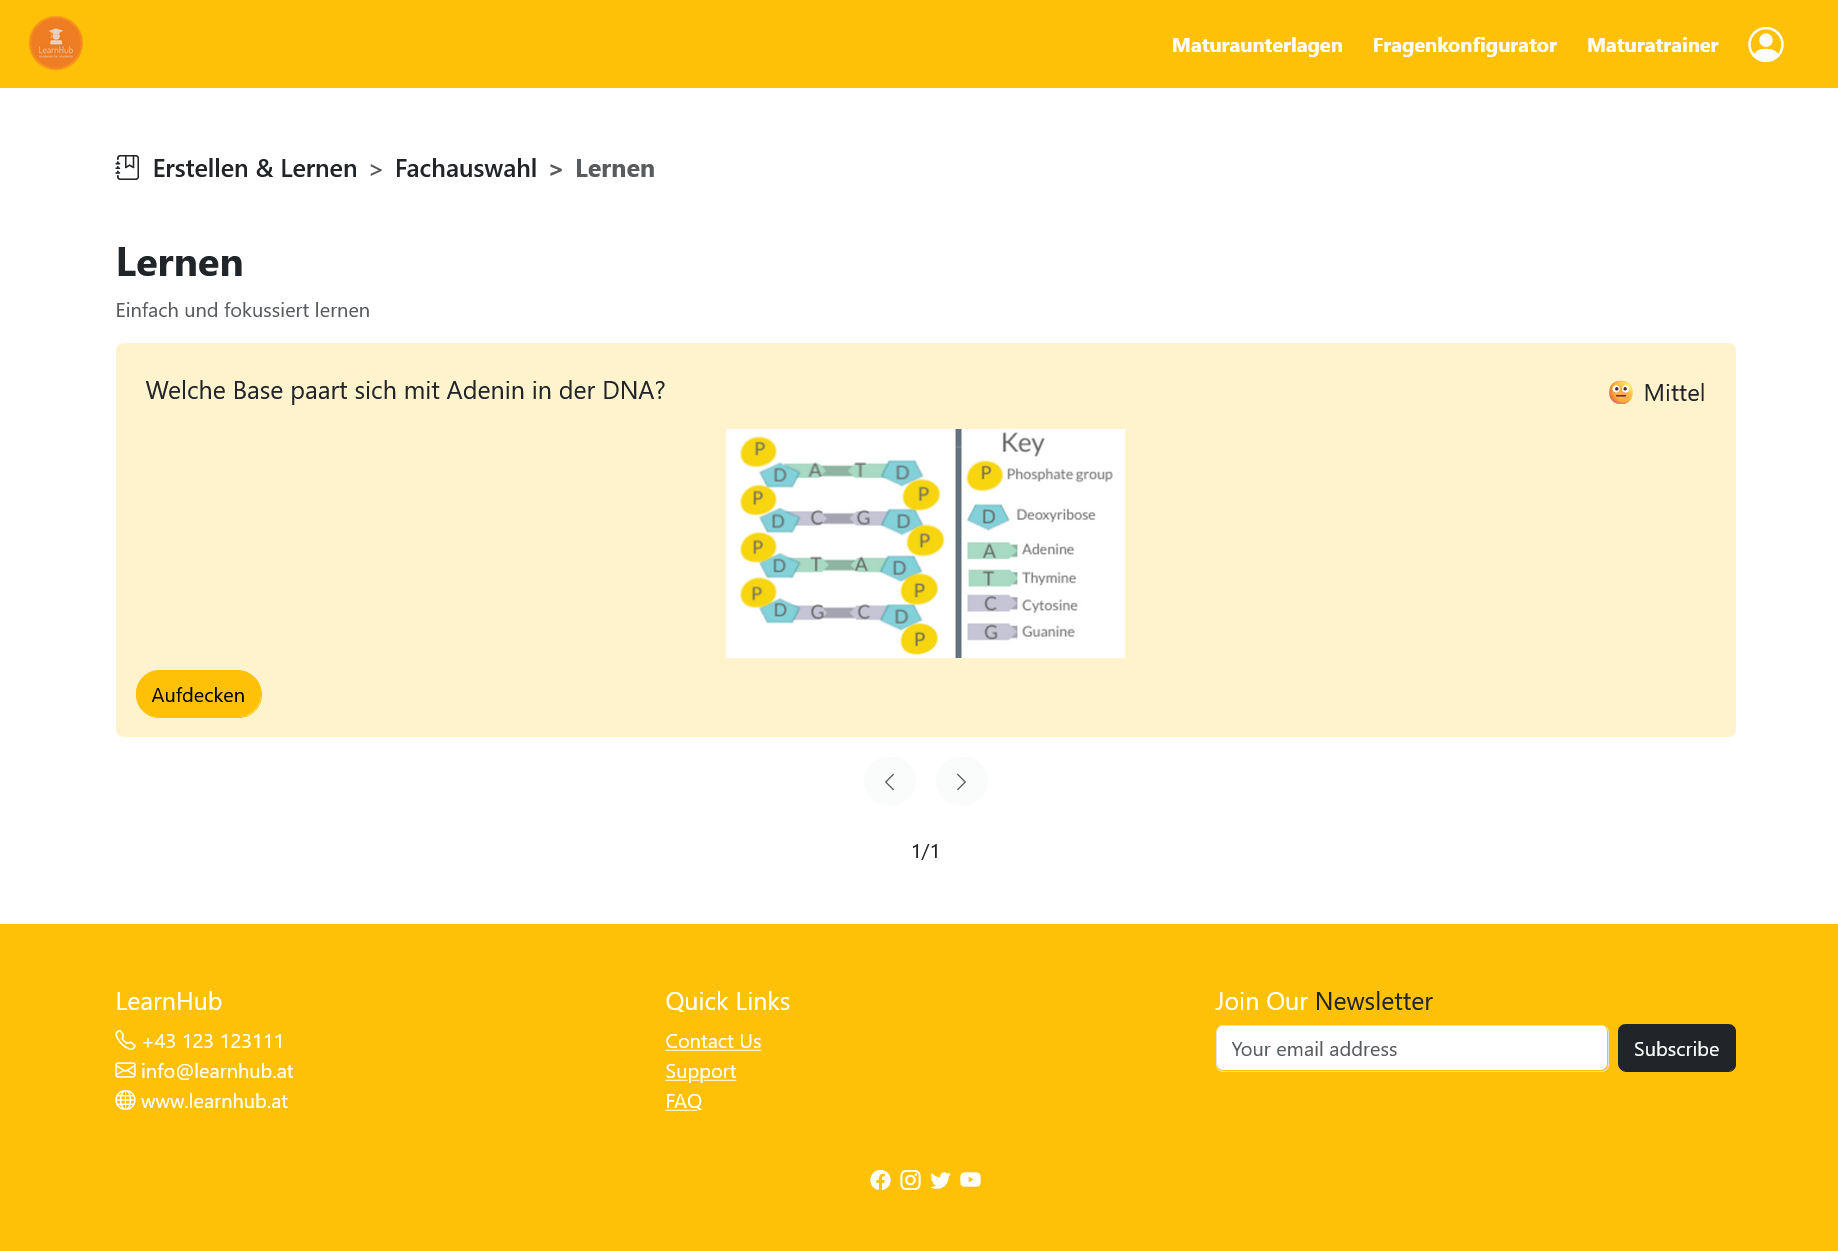
\includegraphics[width=0.6\textwidth]{pics/fragenkonf_lernkarte.png}
    \caption{Lernkarte zugedeckt}
    \label{fig:lernkarte-zugedeckt}
\end{figure}

\subsubsection{Lernmodus} \label{sec:lernmodus}
Im Lernbereich werden die Fragen in Form von hell-orangefarbenen Lernkarten präsentiert. Jede Karte zeigt die Frage, optional ergänzt durch ein Bild. Oben rechts wird der Schwierigkeitsgrad angezeigt: Leicht, Mittel oder Schwer. \par
Unten links befindet sich ein "Aufdecken"-Button. Unter der Karte befinden sich zwei Pfeile zur Navigation durch die Fragen. Darunter wird die aktuelle Frage sowie die Gesamtzahl angezeigt (z.B. 1/12). \par
Durch einen Klick auf den "Aufdecken"-Button kann der/die Nutzer:in die Antwort einsehen.
\begin{figure}[h t]
    \centering
    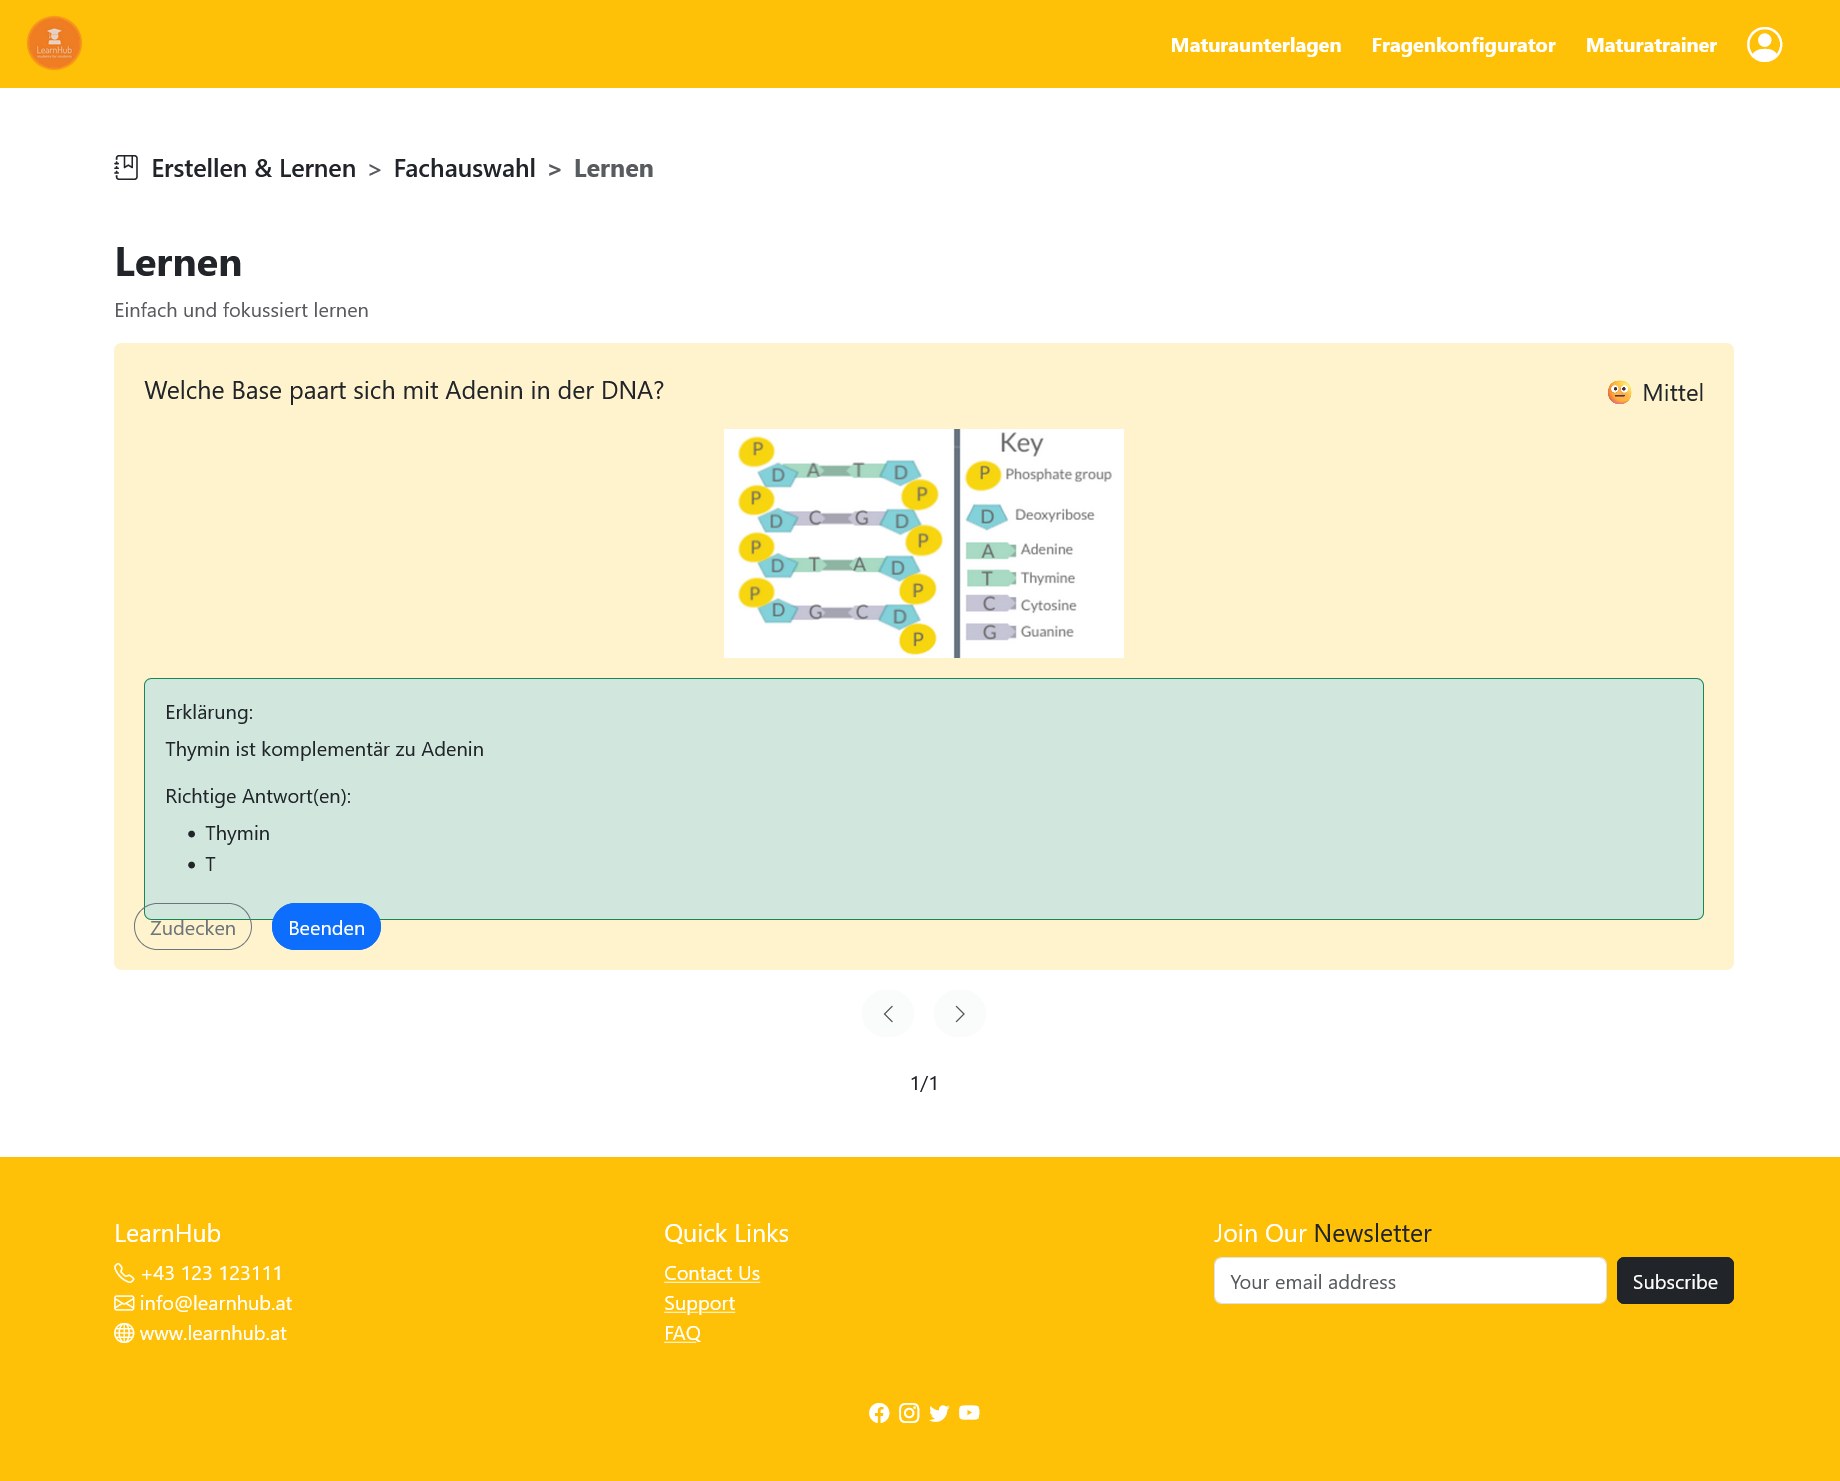
\includegraphics[width=0.6\textwidth]{pics/fragenkonf_lernkarte_aufgedeckt.png}
    \caption{Lernkarte aufgedeckt}
    \label{fig:lernkarte-aufgedeckt}
\end{figure}

\subsubsection{Aufgedeckte Lernkarte}
Nach dem Aufdecken erscheint die Antwort im blauen Bereich. Bei Multiple-Choice-Fragen werden die korrekten Antwortmöglichkeiten und die Erklärung angezeigt. Bei Freitextfragen wird die richtige Antwort oder Erklärung dargestellt.\par
Unter der blauen Box befinden sich zwei Buttons: "Zudecken" (grau) und "Weiter" (blau). Der "Zudecken"-Button verschließt die Karte wieder, während der "Weiter"-Button zur nächsten Frage führt. Bei der letzten Frage ersetzt der "Beenden"-Button den "Weiter"-Button und führt zur Glückwunschseite.\par
\begin{figure}[h t]
    \centering
    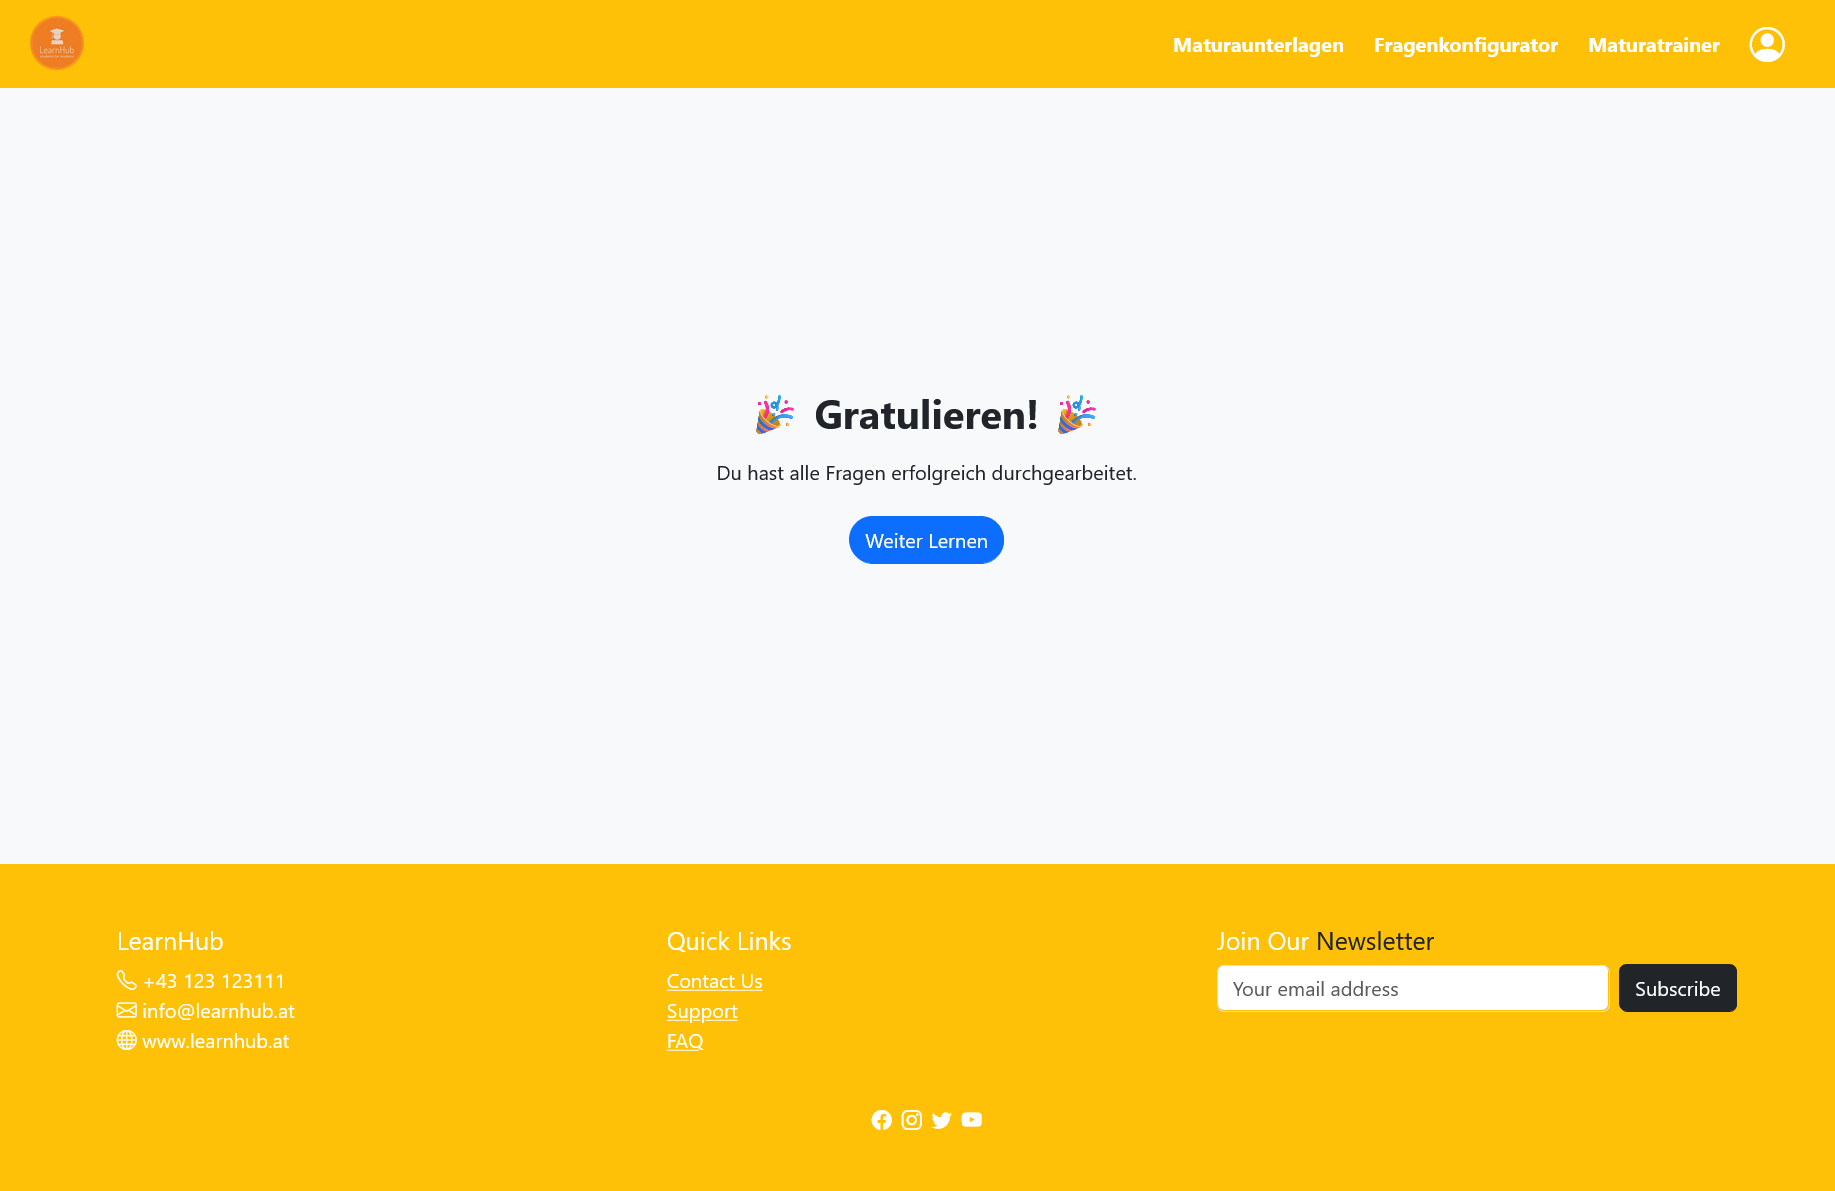
\includegraphics[width=0.6\textwidth]{pics/glueckwunsch.png} 
    \caption{Glückwunschseite nach Beenden des Lernmodus}
    \label{fig:glueckwunsch}
\end{figure}

\subsubsection{Glückwunschseite}
Nach Abschluss des Lernmodus erscheint eine kurze Glückwunschmeldung. Sie informiert den/die Nutzer:in über den erfolgreichen Abschluss und bietet einen Button "Weiter Lernen", über den die Fachauswahl erneut geöffnet werden kann.

\subsection{Fragen verwalten} \label{sec:fragen-verwalten}
\begin{figure}[h t]
    \centering
    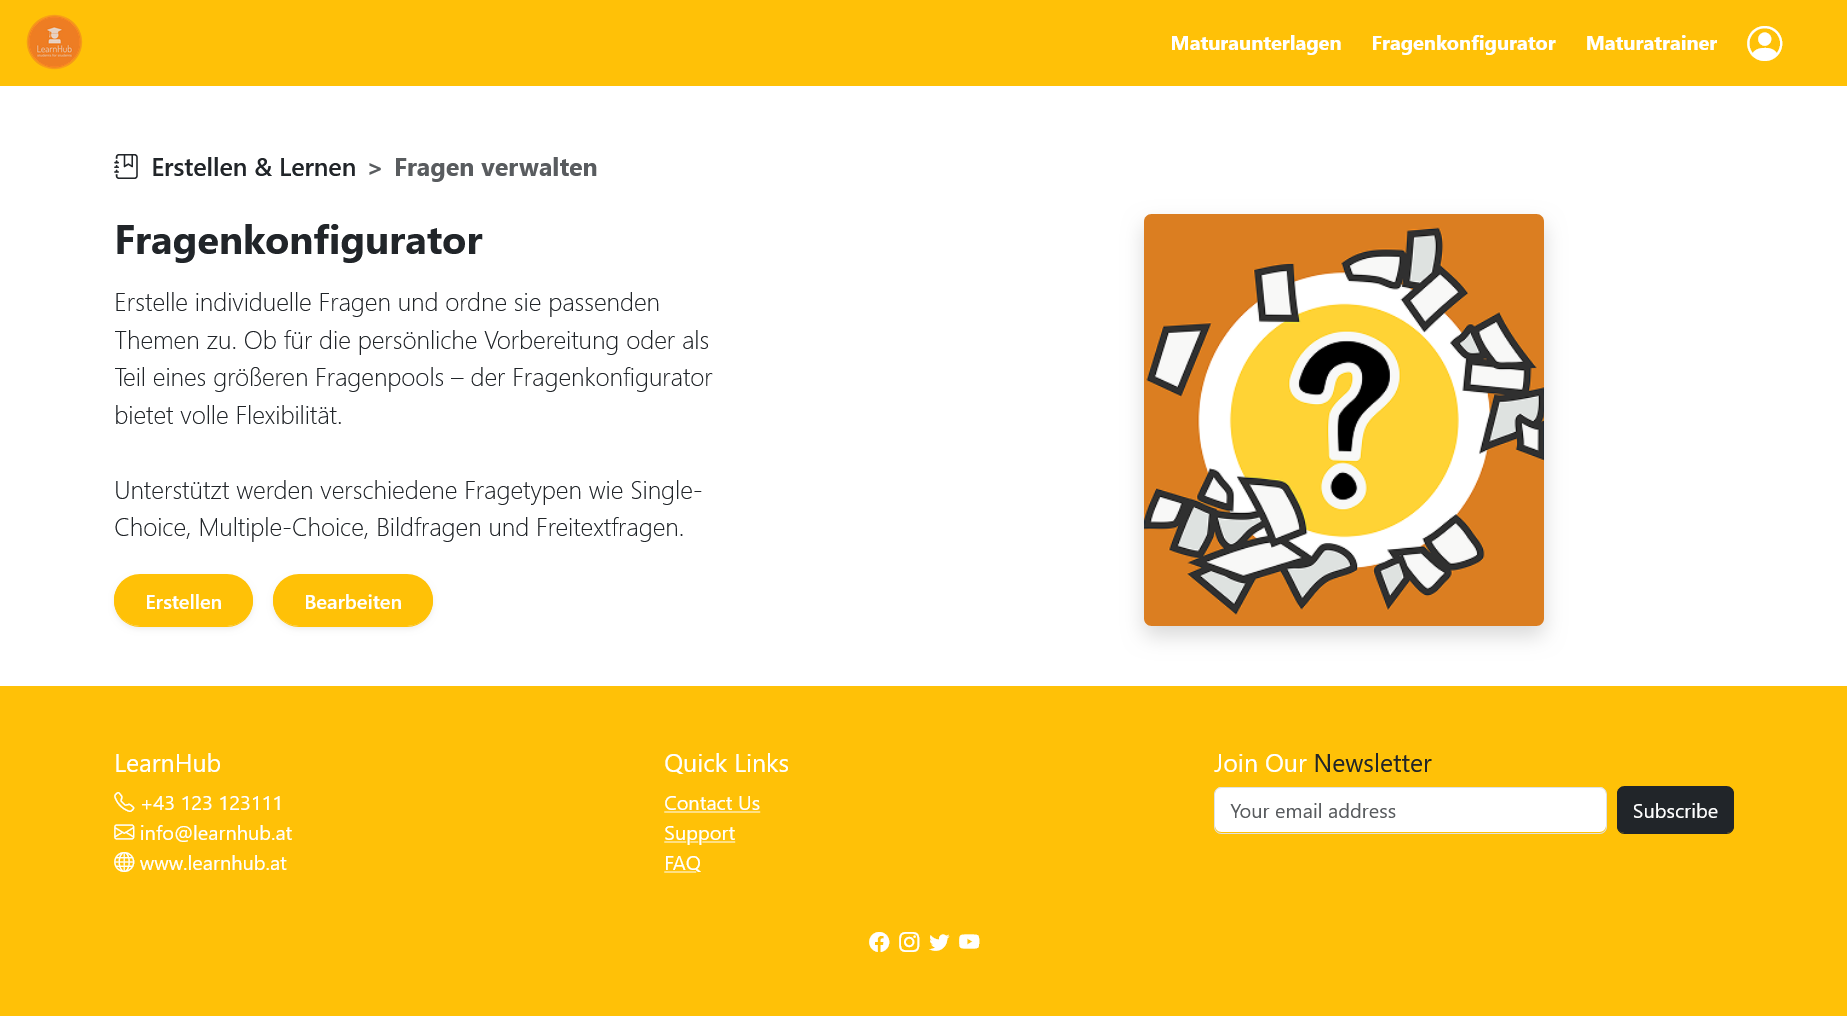
\includegraphics[width=0.6\textwidth]{pics/fragenkonf_erstellen_lernen.png} 
    \caption{Fragen verwalten}
    \label{fig:fragen-vewalten}
\end{figure}

In der Fragenverwaltungsansicht \ref{fig:fragen-verwalten} kann der/die Nutzer:in wählen, ob eine neue Frage erstellt oder eine bestehende Frage bearbeitet werden soll.
Ein Klick auf „Erstellen“ öffnet den Fragenkonfigurator, in dem eine neue Frage formuliert werden kann.
Wird stattdessen „Bearbeiten“ ausgewählt, erscheint eine Liste der bereits vorhandenen Fragen, aus der eine Frage zur Bearbeitung ausgewählt werden kann.

